\documentclass[../notes.tex]{subfiles}

\pagestyle{main}
\renewcommand{\chaptermark}[1]{\markboth{\chaptername\ \thechapter\ (#1)}{}}
\stepcounter{chapter}

\begin{document}




\chapter{Spectrometry}
\section{Office Hours (Snyder)}
\begin{itemize}
    \item \marginnote{1/17:}Does cyclohexane only have one \ce{{}^13C} NMR signal, and only one \ce{{}^1H} NMR signal?
    \begin{itemize}
        \item 1 singlet for \ce{{}^13C}.
        \item 1 singlet for \ce{{}^1H}.
        \item We don't integrate carbon.
        \item We only integrate to compare things.
        \item We won't have to deal with cyclohexane conformations wrt. NMR on any test.
    \end{itemize}
    \item What do we need to know about the Karplus correlation?
    \begin{itemize}
        \item We won't need it for problems.
        \item It's useful, but we've got other things to worry about.
    \end{itemize}
    \item Do chemists/when do chemists run \ce{{}^13C} NMR experiments with all carbons isotopically carbon-13?
    \item Is the reason we don't integrate carbon because the placing of the carbon-13s is random? Would the proportions not still be representative?
    \item For \ce{{}^1H} NMR, feel free to draw in the hydrogen atoms on the line-angle structure.
    \item Multiplying $n+1$ of different types of neighbors (e.g., if a hydrogen has 3 neighboring hydrogens to one side and 2 neighboring hydrogens to the other side, it has a maximum of $(3+1)(2+1)=12$ peaks in its signal).
    \begin{itemize}
        \item The multiplication analysis applies only to chains that are completely different.
    \end{itemize}
\end{itemize}



\section{NMR}
\begin{itemize}
    \item \marginnote{1/18:}With a $\SI{1400}{\mega\hertz}$ NMR spectrometer, we can see 3D structure.
    \item Goes over an example of sketching a \ce{{}^13C} spectrum, DEPT 90, and DEPT 135 spectrum for a given molecule.
    \item You can flip groups in a problem, but you have to be consistent.
    \begin{itemize}
        \item If you have closely spaced peaks in a sketch, be consistent with identifying a certain peak as \ce{CH}, \ce{CH2}, or \ce{CH3}. But it doesn't matter which of the peaks you identify which way.
    \end{itemize}
    \item There can be variation in signal height, but we won't discuss this.
    \item Transition to \ce{{}^1H} NMR spectroscopy.
    \item A typical \ce{{}^13C} NMR experiment takes 1-2 hours (for about $\SI{5}{\milli\gram}$ of material) to build appropriate peaks since there are so few \ce{{}^13C} atoms interspersed.
    \begin{itemize}
        \item On a strong field machine, though, a \ce{{}^1H} spectrum can be done in seconds.
    \end{itemize}
    \item Goes over typical chemical shifts (see Table \ref{tab:protonChemicalShifts}).
    \item Goes over an example of sketching a \ce{{}^1H} spectrum.
    \item Neighboring spins parallel to the magnetic field increase ppm (deshielding).
    \item Introduces the coupling constant $J$.
    \item Splitting can happen in \ce{{}^13C} spectra, but it can't be observed on the time scale on which we measure.
    \item Terminology: Singlet, doublet, triplet, quartet, pentet, and sextet.
    \item Multiple neighbors? Multiply!
    \begin{itemize}
        \item If you have 3 neighbors on one side and 2 on the other, for instance, you will have $(3+1)(2+1)=12$ peaks.
        \item Note that this is our predicted value --- due to overlap, we may see fewer, but we will always go with the predicted value in this class.
    \end{itemize}
    \item Count neighbors even on non-carbon atoms.
    \item Hybridization.
    \begin{itemize}
        \item Don't get bothered by the hybridization of parent carbons if it doesn't restrict conformations. For example, the $sp^2$ carbon in an aldehyde behaves the same as any other parent carbon.
        \item Do worry about hybridization if it makes hydrogens nonequivalent. In 1-butene for example, the two terminal hydrogens on the alkene are nonequivalent.
        \begin{itemize}
            \item We will not worry about multiplicity due to this effect, though the rules are similar to what we've seen.
        \end{itemize}
    \end{itemize}
    \item Benzenes.
    \begin{figure}[h!]
        \centering
        \footnotesize
        \begin{subfigure}[b]{0.2\linewidth}
            \centering
            \chemfig{*6(-(-[,,,,white]\phantom{Cl})=-=(-Br)-=)}\\[1em]
            \begin{tikzpicture}
                \path (0,0) -- (0,1);
                \draw (-1,0) -- (1,0);
    
                \draw [rex,semithick] (-0.5,0)
                    \foreach \x in {-0.45,-0.4,...,0.45} {
                        -- (\x,0.5+0.5*rand)
                    }
                -- (0.5,0);
            \end{tikzpicture}
            \caption{}
            \label{fig:benzeneH1NMRa}
        \end{subfigure}
        \begin{subfigure}[b]{0.2\linewidth}
            \centering
            \chemfig{*6(-(-[,,,,white]\phantom{Cl})=-(-Cl)=(-Br)-(-[,,,,white]\phantom{Cl})=)}\\[1em]
            \begin{tikzpicture}
                \path (0,0) -- (0,1);
                \draw (-1,0) -- (1,0);
    
                \draw [rex,semithick] (-0.5,0)
                    \foreach \x in {-0.45,-0.4,...,0.45} {
                        -- (\x,0.4+0.4*rand)
                    }
                -- (0.5,0);
            \end{tikzpicture}
            \caption{}
            \label{fig:benzeneH1NMRb}
        \end{subfigure}
        \begin{subfigure}[b]{0.2\linewidth}
            \centering
            \chemfig{*6((-[,,,,white]\phantom{Cl})-(-[,,,,white]\phantom{Cl})=(-Cl)-=(-Br)-=)}\\[1em]
            \begin{tikzpicture}
                \path (0,0) -- (0,1);
                \draw (-1,0) -- (1,0);
    
                \draw [rex,semithick] (-0.5,0) -- (-0.45,1) -- (-0.4,0) -- (-0.3,0)
                    \foreach \x in {-0.25,-0.2,...,0.45} {
                        -- (\x,0.3+0.3*rand)
                    }
                -- (0.5,0);
            \end{tikzpicture}
            \caption{}
            \label{fig:benzeneH1NMRc}
        \end{subfigure}
        \begin{subfigure}[b]{0.2\linewidth}
            \centering
            \chemfig{*6(-(-Cl)=-=(-Br)-=)}\\[1em]
            \begin{tikzpicture}
                \path (0,0) -- (0,1);
                \draw (-1,0) -- (1,0);
    
                \draw [rex,semithick] (-0.5,0) -- (-0.45,1) -- (-0.4,0) -- (-0.35,1) -- (-0.3,0) -- (0.3,0) -- (0.35,1) -- (0.4,0) -- (0.45,1) -- (0.5,0);
            \end{tikzpicture}
            \caption{}
            \label{fig:benzeneH1NMRd}
        \end{subfigure}
        \caption{Benzenes in \ce{{}^1H} NMR spectroscopy.}
        \label{fig:benzeneH1NMR}
    \end{figure}
    \begin{itemize}
        \item We can predict a bunch of splitting and peaks, but often there is so much overlap that we more just get a jagged blob (see Figures \ref{fig:benzeneH1NMRa} and \ref{fig:benzeneH1NMRb}).
        \item If you can find a clear singlet, perhaps separated a bit from the rest, integration can tell you how many substituents you have (see Figure \ref{fig:benzeneH1NMRc}).
        \item The pattern in Figure \ref{fig:benzeneH1NMRd} is a dead giveaway for para substituents.
    \end{itemize}
    \item Alkene coupling constants.
    \begin{itemize}
        \item \emph{cis}-alkenes typically have $J=\SIrange{6}{10}{\hertz}$.
        \item \emph{trans}-alkenes typically have $J=\SIrange{12}{18}{\hertz}$.
        \item These are identifiable, diagnostic signals.
    \end{itemize}
    \item Enantiomers are identical in NMR experiments.
    \begin{itemize}
        \item Remember that all of their physical properties are the same (including the various forms of spectroscopy) except optical rotation.
    \end{itemize}
\end{itemize}



\section{Chapter 9: Nuclear Magnetic Resonance and Mass Spectroscopy}
\emph{From \textcite{bib:SolomonsEtAl}.}
\begin{itemize}
    \item \textbf{Mass spectrometry}: The formation of ions in a mass spectrometer followed by separation and detection of the ions according to mass and charge.
    \item \textbf{Mass spectrum}: A graph that on the $x$-axis represents the formula weights of the detected ions, and on the $y$-axis represents the abundance of each detected ion.
    \begin{figure}[h!]
        \centering
        \begin{tikzpicture}[xscale=0.2,yscale=0.05]
            \draw [xstep=10cm,ystep=20cm,gax,semithick] (10,0) grid (50,100);
            \foreach \y in {10,30,...,90} {
                \draw (10,\y) -- ++(1,0) ++(38,0) -- ++(1,0);
            }
    
            \small
            \node [rotate=90,above=7mm] at (10,50) {Relative Ion Abundance};
            \node [below=5mm] at (30,0) {$m/z$};
    
            \footnotesize
            \foreach \x in {10,20,...,50} {
                \node [below] at (\x,0) {$\x$};
            }
            \node [above left] at (10,0) {$0$};
            \foreach \y in {20,40,...,100} {
                \node [left] at (10,\y) {$\y$};
            }
    
            \draw [orx,ultra thick]
                % 
                (45,0) -- ++(0,1)
                (44,0) -- ++(0,28)
                (43,0) -- ++(0,24)
                (42,0) -- ++(0,7)
                (41,0) -- ++(0,14)
                (40,0) -- ++(0,3)
                (39,0) -- ++(0,20)
                (38,0) -- ++(0,6)
                (37,0) -- ++(0,3)
                (36,0) -- ++(0,1)
                (30,0) -- ++(0,3)
                (29,0) -- ++(0,100)
                (28,0) -- ++(0,59)
                (27,0) -- ++(0,42)
                (26,0) -- ++(0,10)
                (25,0) -- ++(0,0.5)
                (24,0) -- ++(0,0.5)
                (21,0) -- ++(0,0.5)
                (20,0) -- ++(0,1)
                (19,0) -- ++(0,1)
                (16,0) -- ++(0,1)
                (15,0) -- ++(0,7)
                (14,0) -- ++(0,3)
                (13,0) -- ++(0,1)
                (12,0) -- ++(0,1)
            ;
        \end{tikzpicture}
        \caption{The mass spectrum of propane.}
        \label{fig:MSpropane}
    \end{figure}
    \begin{itemize}
        \item The $x$-axis is labeled $m/z$ where $m$ is mass and $z$ is charge.
        \item The examples \textcite{bib:SolomonsEtAl} consider all have $z=+1$, so the $x$-axis in them effectively represents the formula weight of each detected ion.
    \end{itemize}
    \item \textbf{Base peak}: The tallest peak in a mass spectrum.
    \begin{itemize}
        \item Relative ion abundance on the $y$-axis is either expressed as a percentage of the base peak or directly as the number of detected ions.
        \item Usually an easily formed fragment of the original compound.
        \item The base peak in Figure \ref{fig:MSpropane} corresponds to the \ce{C2H5+} ion, $m/z=29=2\cdot 12+5\cdot 1$.
    \end{itemize}
    \item \textbf{Molecular ion}: The ion with the formula weight of the original compound.
    \begin{itemize}
        \item One of the higher value $m/z$ peaks.
        \item Usually not the base peak.
    \end{itemize}
    \item Small peaks having $m/z$ values 1 or 2 higher than the formula weight of the compound are due to \ce{{}^13C} and other isotopes.
    \item \textbf{Electron impact}: A method for ionizing molecules in a mass spectrometer by placing the sample under high vacuum and bombarding it with a beam of high-energy electrons. \emph{Also known as} \textbf{EI}.
    \begin{itemize}
        \item The energy of the electrons is in the range of $\SI{70}{\electronvolt}$ or $\SI[per-mode=symbol]{6.7e3}{\kilo\joule\per\mole}$.
        \item The incoming electrons ionize the molecules to molecular ions, which are radical cations since they have a $+1$ charge and an unshared electron.
    \end{itemize}
    \item Note that there are ionization methods other than EI, but it is the most common.
    \item Localizing the radical and charge along the structure.
    \begin{figure}[h!]
        \centering
        \footnotesize
        \begin{subfigure}[b]{0.24\linewidth}
            \centering
            \ce{[CH3CH2CH3]+}\hspace{-4.8pt}.
            \caption{Propane.}
            \label{fig:molecularIonsa}
        \end{subfigure}
        \begin{subfigure}[b]{0.24\linewidth}
            \centering
            \chemfig{CH_3-\charge{-90=\:,73={\tiny$+$},107=\.}{O}H}
            \caption{Methanol.}
            \label{fig:molecularIonsb}
        \end{subfigure}
        \begin{subfigure}[b]{0.24\linewidth}
            \centering
            \chemfig{CH_3-\charge{-73={\tiny$+$},-107=\.}{N}(-[2]CH_3)-CH_3}
            \caption{Trimethylamine.}
            \label{fig:molecularIonsc}
        \end{subfigure}
        \begin{subfigure}[b]{0.24\linewidth}
            \centering
            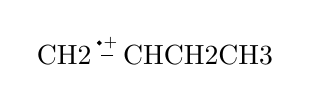
\begin{tikzpicture}
                \node (1) {\ce{CH2}};
                \node (2) at (1.7,0) {\ce{CHCH2CH3}}
                    edge node[above=-1pt]{\tikz[baseline={(0,-0.04)}]{\filldraw circle (0.15ex);}\hspace{0.6pt}{\tiny$+$}} (1)
                ;
            \end{tikzpicture}
            \caption{1-Butene.}
            \label{fig:molecularIonsd}
        \end{subfigure}
        \caption{Molecular ions.}
        \label{fig:molecularIons}
    \end{figure}
    \begin{itemize}
        \item The choice of where we localize the radical/charge is often arbitrary (esp. with hydrocarbons).
        \item However, "as we might expect, ionization potentials indicate that in [the] formation of radical cations, the nonbonding electrons of nitrogen, oxygen, and halogen atoms, and the $\pi$ electrons of alkenes and aromatic molecules, are held more loosely than the electrons of carbon-carbon and carbon-hydrogen $\sigma$ bonds" \parencite[425]{bib:SolomonsEtAl}.
        \item Thus, "when a molecule contains oxygen, nitrogen, or a $\pi$ bond, we place the odd electron and charge at a nitrogen, oxygen, halogen, or $\pi$ bond. If resonance is possible, the radical cation may be delocalized" \parencite[425]{bib:SolomonsEtAl}.
    \end{itemize}
    \item Three important principles.
    \begin{enumerate}
        \item The reactions that take place are all unimolecular since the pressure is kept so low.
        \item Single-barbed arrows denote the movement of single electrons.
        \item The relative ion abundances give key information about the structures of the fragments produced and their original locations in the molecule.
    \end{enumerate}
    \item Fragmentation by cleavage at a single bond.
    \begin{itemize}
        \item When such a process happens in a molecular ion, a cation and a radical are produced, although only the cation will be detected by the positive ion mass spectrometers we're considering.
        \item Each cleavage can happen in two ways (since one fragment will take the radical and the other will take the positive charge).
        \item The path that produces the more stable carbocation will occur more rapidly.
        \begin{itemize}
            \item Notice the difference in relative ion abundance between the secondary \ce{CH3CH2+} ($m/z=29$) and the primary \ce{CH3+} ($m/z=15$) in Figure \ref{fig:MSpropane}.
        \end{itemize}
    \end{itemize}
    \item When drawing cleavage reactions, use brackets and delocalization; when drawing cleavage mechanisms, use localization.
    \item Chain branching increases the likelihood of cleavage at a branch point because a more stable carbocation can result.
    \item Examples of fragmentation to form resonance-stabilized cations.
    \begin{enumerate}
        \item Alkenes ionize and frequently undergo fragmentations that yield resonance-stabilized allylic cations.
        \begin{figure}[h!]
            \centering
            \footnotesize
            \schemestart
                \chemfig{CH_2=CH-CH_2-R}
                \arrow{->[ionization][-$\e[-]$]}[,1.4]
                \chemfig{CH_2-[@{db2},,,,lddbond]CH-[@{sb2a}]CH_2-[@{sb2b}]@{R2}R}
                \arrow{->[fragmentation]}[,1.8]
                \chemleft{[}
                    \subscheme{
                        \chemfig{\charge{90={\tiny$+$}}{C}H_2-CH=CH_2}
                        \arrow(.south--.north){<->}[-90]
                        \chemfig{CH_2=CH-\charge{90={\tiny$+$}}{C}H_2}
                    }
                \chemright{]}
                \arrow{0}[,0]\+
                \chemfig{\charge{180=\.}{R}}
            \schemestop
            \chemmove{
                \draw [rex,semithick,shorten <=4pt,shorten >=2pt,arrows={-Stealth[harpoon,swap]}] (db2) to[bend left=60,looseness=1.5] (sb2a);
                \draw [rex,semithick,shorten <=2pt,shorten >=2pt,arrows={-Stealth[harpoon]}] (sb2b) to[bend right=60,looseness=1.5] (sb2a);
                \draw [rex,semithick,shorten <=2pt,shorten >=2pt,arrows={-Stealth[harpoon,flex]}] (sb2b) to[bend left=60,looseness=1.5] (R2);
            }
            \caption{Resonance fragmentation: Alkenes.}
            \label{fig:resonanceFragAlkene}
        \end{figure}
        \item Carbon-carbon bonds next to an atom with a lone pair usually break readily because the resulting carbocation is resonance stabilized.
        \begin{figure}[h!]
            \centering
            \footnotesize
            \schemestart
                \chemfig{R-\charge{90=\:}{Z}-CH_2-CH_3}
                \arrow{->[ionization][-$\e[-]$]}[,1.4]
                \chemfig{R-@{Z2}\charge{73=\.,107={\tiny$+$}}{Z}-[@{sb2a}]CH_2-[@{sb2b}]@{C2}CH_3}
                \arrow{->[fragmentation]}[,1.8]
                \chemleft{[}
                    \subscheme{
                        \chemfig{R-\charge{90={\tiny$+$}}{Z}=CH_2}
                        \arrow(.south--.north){<->}[-90]
                        \chemfig{R-\charge{90=\:}{Z}-\charge{90={\tiny$+$}}{C}H_2}
                    }
                \chemright{]}
                \arrow{0}[,0]\+
                \chemfig{\charge{180=\.}{C}H_3}
            \schemestop
            \chemmove{
                \draw [rex,semithick,shorten <=6pt,shorten >=2pt,arrows={-Stealth[harpoon,swap]}] (Z2) to[bend left=80,looseness=3] (sb2a);
                \draw [rex,semithick,shorten <=2pt,shorten >=2pt,arrows={-Stealth[harpoon]}] (sb2b) to[bend right=60,looseness=1.5] (sb2a);
                \draw [rex,semithick,shorten <=2pt,shorten >=2pt,arrows={-Stealth[harpoon,flex]}] (sb2b) to[bend left=60,looseness=1.5] (C2);
            }
            \caption{Resonance fragmentation: Lone pairs.}
            \label{fig:resonanceFragLonepair}
        \end{figure}
        \item Carbon-carbon bonds next to the carbonyl group of an aldehyde or ketone break readily because resonance-stabilized ions called \textbf{acylium ions} are produced.
        \begin{figure}[h!]
            \centering
            \footnotesize
            \schemestart
                \chemfig{C(-[:120]R)(-[:-120]R')=\charge{[extra sep=1.5pt]45=\:,-45=\:}{O}}
                \arrow{->[ionization][-$\e[-]$]}[,1.4]
                \chemfig{C(-[@{sb2}:120]@{R2}R)(-[:-120]R')=[@{db2}]@{O2}\charge{107=\.,73={\tiny$+$},0=\:}{O}}
                \arrow{->[fragmentation]}[,1.8]
                \chemname{
                    \chemleft{[}
                        \subscheme{
                            \chemfig{R'-C~\charge{90={\tiny$+$},0=\:}{O}}
                            \arrow(.south--.north){<->}[-90]
                            \chemfig{R'-\charge{90={\tiny$+$}}{C}=\charge{[extra sep=1.5pt]45=\:,-45=\:}{O}}
                        }
                    \chemright{]}
                }{Acylium ion}
                \arrow{0}[,0]\+
                \chemfig{\charge{0=\.}{R}}
            \schemestop
            \chemmove{
                \draw [rex,semithick,shorten <=2pt,shorten >=2pt,arrows={-Stealth[harpoon,swap,flex]}] (sb2) to[bend right=60,looseness=1.5] (R2);
                \draw [rex,semithick,shorten <=2pt,shorten >=2pt,arrows={-Stealth[harpoon,swap]}] (sb2) to[bend left=50,looseness=1.3] (db2);
                \draw [rex,semithick,shorten <=6pt,shorten >=2pt,arrows={-Stealth[harpoon,flex]}] (O2) to[bend right=70,looseness=2.5] (db2);
            }
            \caption{Resonance fragmentation: Carbonyls.}
            \label{fig:resonanceFragCarbonyl}
        \end{figure}
        \begin{itemize}
            \item Note that either the \ce{C-R} or the \ce{C-R$'$} bond could break.
        \end{itemize}
        \item Alkyl substituted benzenes ionize by loss of a $\pi$ electron and undergo loss of a hydrogen atom or methyl group to yield the relatively stable \textbf{tropylium ion}. This fragmentation gives a prominent peak (sometimes the base peak) at $m/z=91$.
        \begin{figure}[H]
            \centering
            \footnotesize
            \setchemfig{autoreset cntcycle=false}
            \begin{subfigure}[b]{\linewidth}
                \centering
                \schemestart
                    \chemfig{*6(-=-(-CH_3)=-=)}
                    \arrow{->[ionization][-$\e[-]$]}[,1.4]
                    \chemfig{**6(---(-CH_3)---)}
                    \arrow{->[\shortstack{fragmentation and\\rearrangement}][-\ce{H*}]}[,2.2]
                    \chemname[-3.5em]{
                        \chemfig{[:-12.86]*7(-=-=-@{C3}-=)}
                    }{Tropylium ion}
                \schemestop
                \chemmove{
                    \node at (cyclecenter2) {\tiny$+$\hspace{0.6pt}\tikz[baseline={(0,-0.04)}]{\filldraw circle (0.15ex);}};
                    \node [below] at (C3) {\tiny$+$};
                }
                \caption{Losing a hydrogen radical.}
                \label{fig:resonanceFragBenzeneAlkyla}
            \end{subfigure}\\[2.5em]
            \begin{subfigure}[b]{\linewidth}
                \centering
                \schemestart
                    \chemfig{**6(------)}
                    \arrow{->[\shortstack{fragmentation and\\rearrangement}][-\ce{CH3*}]}[,2.2]
                    \chemfig{[:-12.86]**7(-------)}
                \schemestop
                \chemmove{
                    \node (M1) [at=(cyclecenter4),shift=(60:1)] {\printatom{CH_3}};
                    \node (M2) [at=(cyclecenter4),shift=(-60:1)] {\printatom{CH_3}};
                    \draw [-,shorten <=3pt] (cyclecenter4) -- (M1);
                    \draw [-,shorten <=3pt] (cyclecenter4) -- (M2);
                    \node at (cyclecenter4) {\tiny$+$\hspace{0.6pt}\tikz[baseline={(0,-0.04)}]{\filldraw circle (0.15ex);}};
                    \node at (cyclecenter5) {\tiny$+$};
                }
                \vspace{1em}
                \caption{Losing a methyl radical.}
                \label{fig:resonanceFragBenzeneAlkylb}
            \end{subfigure}
            \caption{Resonance fragmentation: Alkyl-substituted benzene rings.}
            \label{fig:resonanceFragBenzeneAlkyl}
        \end{figure}
        \item Monosubstituted benzenes with other than alkyl groups also ionize by loss of a $\pi$ electron and then lose their substituent to yield a phenyl cation with $m/z=77$.
        \begin{figure}[h!]
            \centering
            \footnotesize
            \setchemfig{autoreset cntcycle=false}
            \schemestart
                \chemfig{[:-30]*6(-=-(-Y)=-=)}
                \arrow{->[ionization][-$\e[-]$]}[,1.4]
                \chemfig{[:-30]**6(---(-[@{sb2}]@{Y2}Y)---)}
                \arrow{->[fragmentation][-\ce{Y}]}[,1.8]
                \chemfig{[:-30]**6(---@{C3}---)}
            \schemestop
            \chemmove{
                \node at (cyclecenter2) {\tiny$+$\hspace{0.6pt}\tikz[baseline={(0,-0.04)}]{\filldraw circle (0.15ex);}};
                \node [right] at (C3) {\tiny$+$};
                \draw [rex,semithick,shorten <=2pt,shorten >=2pt] (sb2) to[bend left=90,looseness=3] (Y2);
            }
            \caption{Resonance fragmentation: Monosubstituted benzene rings with nonalkyl groups.}
            \label{fig:resonanceFragBenzene}
        \end{figure}
        \begin{itemize}
            \item \ce{Y} is a halogen, nitro group, acyl group, nitrile group, etc.
        \end{itemize}
    \end{enumerate}
    \item Fragmentation by cleavage of two bonds leads to a new radical cation and a neutral molecule.
    \begin{enumerate}
        \item Alcohols frequently show a peak at $\ce{M+}\hspace{-4.8pt}.-18$. This corresponds to the loss of a molecule of water.
        \begin{figure}[h!]
            \centering
            \footnotesize
            \schemestart
                \chemfig{R-CH(-[@{sb1a}2]H)-[@{sb1b}]CH_2-[@{sb1c,0.2}2]@{O1}\charge{90=\:,163={\tiny$+$},197=\.}{O}H}
                \arrow(.-18--)
                \chemleft{[}
                    \chemfig{R-CH-[,,,,lddbond]CH_2}
                \chemright{]^+}
                \+
                \chemfig{H-\charge{90=\:,-90=\:}{O}-H}
            \schemestop
            \chemmove{
                \draw [rex,semithick,shorten <=2pt,shorten >=6pt,arrows={-Stealth[harpoon]}] (sb1a) to[out=135,in=150,out looseness=3] (O1);
                \draw [rex,semithick,shorten <=2pt,shorten >=2pt,arrows={-Stealth[harpoon]}] (sb1a) to[bend left=60,looseness=1.5] (sb1b);
                \draw [rex,semithick,shorten <=2pt,shorten >=2pt] (sb1c) to[out=30,in=-60,looseness=1.5] (O1);
            }
            \caption{Fragmentation: Loss of \ce{H2O}.}
            \label{fig:fragH2O}
        \end{figure}
        \item Carbonyl compounds with a hydrogen on their $\gamma$ carbon undergo a fragmentation called the McLafferty rearrangement.
        \begin{figure}[H]
            \centering
            \footnotesize
            \schemestart
                \chemfig{Y-[:30]C(=[@{db1}2]\charge{[extra sep=1.5pt]45=\:,118:1pt={\tiny$+$},152=\.}{O})-[@{sb1a}:-30]\chembelow{C}{\hspace{5pt}H_2}-[@{sb1b}:30]CH_2-[@{sb1c}2]CH(-[@{sb1d}:150]@{H1}H)-[:30,,1]R}
                \arrow
                \chemfig{Y-[:30]C(-[2]\charge{90=\:,197={\tiny$+$},163=\.}{O}-[:30]H)=[:-30]CH_2}
                \arrow{0}[,0]\+{1em,1em,2em}
                \chemfig{CH_2=[2]CH-[:30,,1]R}
            \schemestop
            \chemmove{
                \draw [rex,semithick,shorten <=3pt,shorten >=2pt] (db1) to[bend right=50,looseness=1.4] (H1);
                \draw [rex,semithick,shorten <=2pt,shorten >=2pt] (sb1b) to[bend right=60,looseness=1.5] (sb1a);
                \draw [rex,semithick,shorten <=2pt,shorten >=2pt] (sb1d) to[bend right=60,looseness=1.5] (sb1c);
            }
            \vspace{1em}
            \caption{Fragmentation: McLafferty rearrangement.}
            \label{fig:fragMcLafferty}
        \end{figure}
        \begin{itemize}
            \item \ce{Y} may be an alkyl, hydride, ether, hydroxyl, etc.
        \end{itemize}
        \item There are also often peaks corresponding to the elimination of other small molecules.
    \end{enumerate}
    \item Isotope effects:
    \begin{itemize}
        \item The presence of \ce{{}^13C} will provide a small peak at $\ce{M+}\hspace{-4.8pt}.+1$.
        \item "In the mass spectrum for a sample containing chlorine, we would expect to find peaks separated by two mass units, in an approximately $3:1$ ($75.5\%:24.5\%$) ratio for the molecular ion or any fragments that contain chlorine" \parencite[432]{bib:SolomonsEtAl}.
        \item "In the mass spectrum for a sample containing bromine, we would expect to find peaks separated by two mass units in an approximately $1:1$ ratio ($50.5\%:49.5\%$ \ce{{}^79Br} to \ce{{}^81Br})" \parencite[433]{bib:SolomonsEtAl}.
        \item In a molecule containing two bromine atoms, for example, we'll see peaks at $\ce{M+}\hspace{-4.8pt}.$, $\ce{M+}\hspace{-4.8pt}.+2$, and $\ce{M+}\hspace{-4.8pt}.+4$ in a $1:2:1$ ratio.
    \end{itemize}
\end{itemize}




\end{document}